%!TEX root = ../report.tex
\documentclass[../report.tex]{subfiles}
\begin{document}
    \chapter{Methodology}
	Last chapter gave a literature review of different attribution methods considered for our research work. This chapter explains the methodical approach taken to address the research problem at hand, by discussing the design of experiments and rationale behind different choices made to conduct them. 
	\section{Datasets}
	This research work uses two datasets for conducting experiments. Frontal facial images of patients with rare genetic syndrome are taken from the GestaltMatcher DataBase (GMDB) dataset. The dataset contains 12849 facial images from 7640 patients with 742 different syndromes. Besides patient images, the dataset also contains other details such as patient history. GMDB acts a valuable resource for the research community.\\
	The UTKFace \cite{zhifei2017cvpr} is used for the dataset imbalance - explanation quality experiment   \ref{sec_data_imb} that requires faces from a healthy cohort. The dataset has over 20,000 face images with labels for age, gender and ethnicity. For the experiment, we handpick 244 samples from the dataset, while ensuring the diversity of the dataset.
	      
    \section{Selection of Methods}\label{sec_method_selection}
    In this section, we analyze the neural network explainability methods dicussed in Chapter 2 based on the following dimensions and identify the ones to be considered for further experimentation and evaluation:
    \begin{itemize}
    	\item \textbf{Saturation problem:} As briefly described in \ref{sec_saturation}, saturation problem occurs when the output of a neural network model gets saturated and its gradients with respect to inputs become insensitive, thereby affecting the quality of generated attribution maps. Shrikumar et al. \cite{shrikumar2017learning} reported that occlusion sensitivity maps, layer-wise relevance propagation, saliency maps, guided-backpropation and guided-GradCAM methods suffer from this problem. Besides, they also report the failure of deconvolution approach in the presence of discontinuos input gradients.   
    	\item \textbf{Sensitivity to changes in model and data:} Adebayo et al. \cite{adebayo2018sanity} investigated faithfulness of explanations produced by popular attribution methods. The chosen methods were evaluated based on their sensitivity to randomization induced in the considered neural network model's weights and labels of the training instances. Authors report that guided-backpropagation and guided-GradCAM remained insensitive to the changes in model and data, having functioned merely as edge detectors. GradCAM passed this sanity check.
    	\item \textbf{Robustness of explanations:} An interpretability method is robust when it generate similar explanations for similar inputs. David Alvarez et al. \cite{alvarez2018robustness} and Yi-han Sheu \cite{sheu2020illuminating} reported that DeepLIFT experiences robustness issues and produces inaccurate results in the presence of multiplicative interactions between features. Besides the lack of robustness, the success of DeepLIFT depends on factors such the choice of reference/baseline image, which is difficult to determine. 
    	\item \textbf{Relevance to the problem at hand:} Along with the above list dimensions, this work shortlists the methods based on their ability to produce meaningful explanations in the context of genetic syndrome recognition. Figures \ref{example_ipa} and \ref{example_la}  shows few sample attribution maps generated from applying both the considered sets of input and layer attribution maps to the GestaltMatcher model. It can be observed that contours of regions in attribution maps produced by layer attribution methods closely match the scales of phenotypic features of genetic syndromes and parts of human face, in general. This effect is possibly due to the inherent working principles of the two classes of attribution methods.\\
    	Layer attribution maps are obtained by scaling and superimposing feature map activations of the last convolutional layers of a CNN, which are responsible for extracting high-level features from a given input image. This nature makes them more suitable for the problem at hand than input attribution methods, which represent pixel-wise attribution methods.
    \end{itemize}
	
    \subsection{More Reasons to Consider Layer Attribution Methods}
    In addition to the above discussed reasons, it is also observed that layer attribution approaches like GradCAM are widely used to explain neural network models for medical diagnosis \cite{} \cite{} \cite{}. However, the downside of GradCAM is it approaches
    attribution as weakly supervised segmenation problem and \enquote{sometimes higlight locations the model didnot actually use}\cite{draelos2020hirescam}. HiResCAM \cite{draelos2020hirescam}, a recent successor of GradCAM overcomes this issue and produces more faithfulness explanations. Therefore, the method is included in the scope of this work.\\
    GradCAM and HiResCAM are layer-specific and therefore their explanations are limited by the choice of the convolutional layers made. FullGrad \cite{srinivas2019full} overcomes this deficit by considering attributions across all neuronal units of a model and thus becomes a candidate for experimentation. Along with these CAM techniques, occlusion sensitivity mapping is included as a reference explanation method, to better understand the classifier model's regions of attention.
    \begin{figure}[H]
		\hspace*{-2cm}    
    	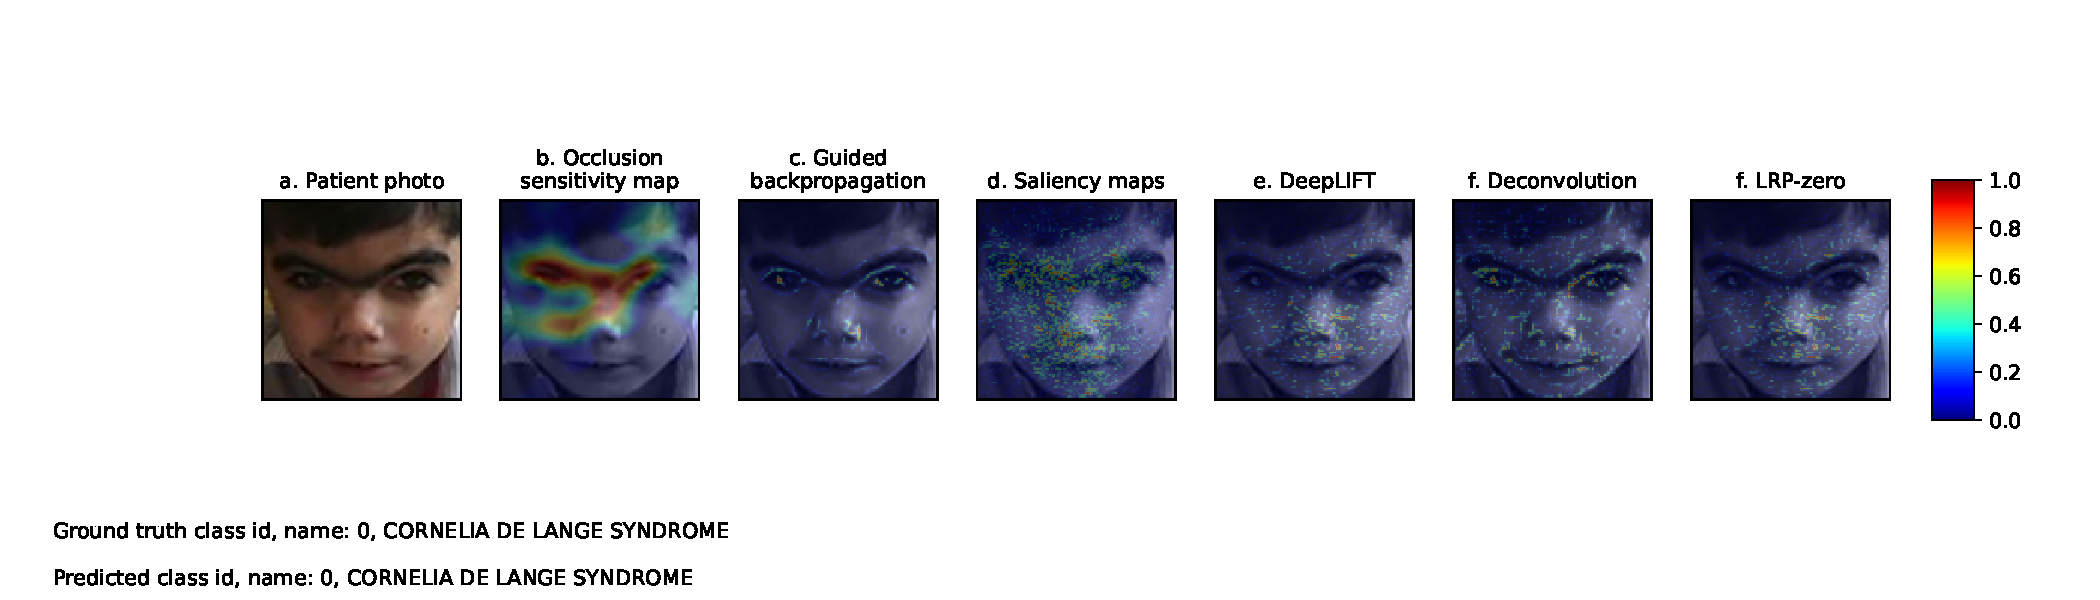
\includegraphics[scale=0.55,trim = 1cm 2.50cm 1cm 2.50cm, clip]{chapter4/input_example.pdf}
    	\caption{An example showing input attribution maps of discussed methods, generated for a patient image}
    	\label{example_ipa}
    	 \vspace{1cm}
    	\hspace*{-1.0cm}    
    	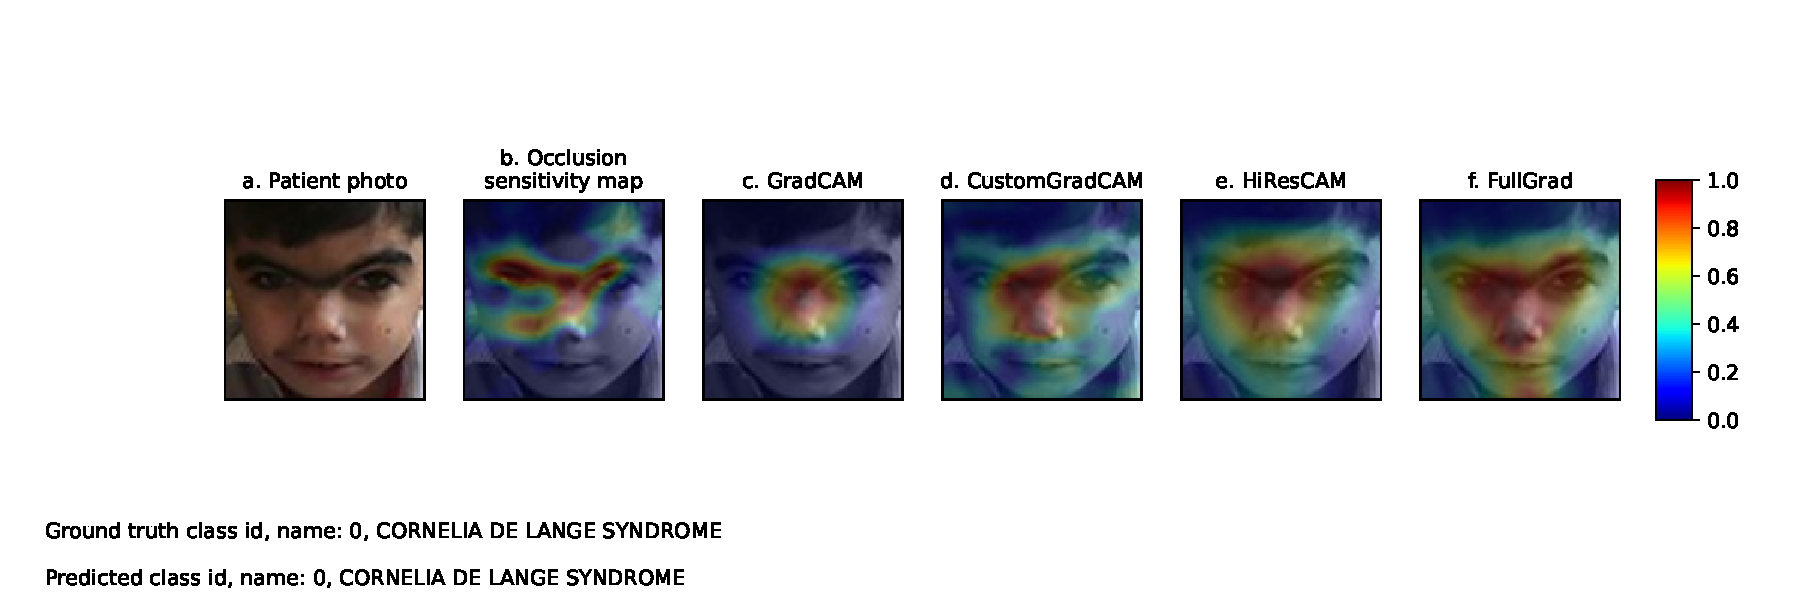
\includegraphics[scale=0.58,trim = 1cm 2.50cm 1cm 2.50cm, clip]{chapter4/layer_example.pdf}
    	\caption{An example for layer attribution maps of discussed methods, generated for a patient image}
    	\label{example_la}
    \end{figure}
    \section{Design of Experiments}\label{sec_exp_design}
    \begin{figure}[ht]
    	\hspace*{-0.5cm}      
       	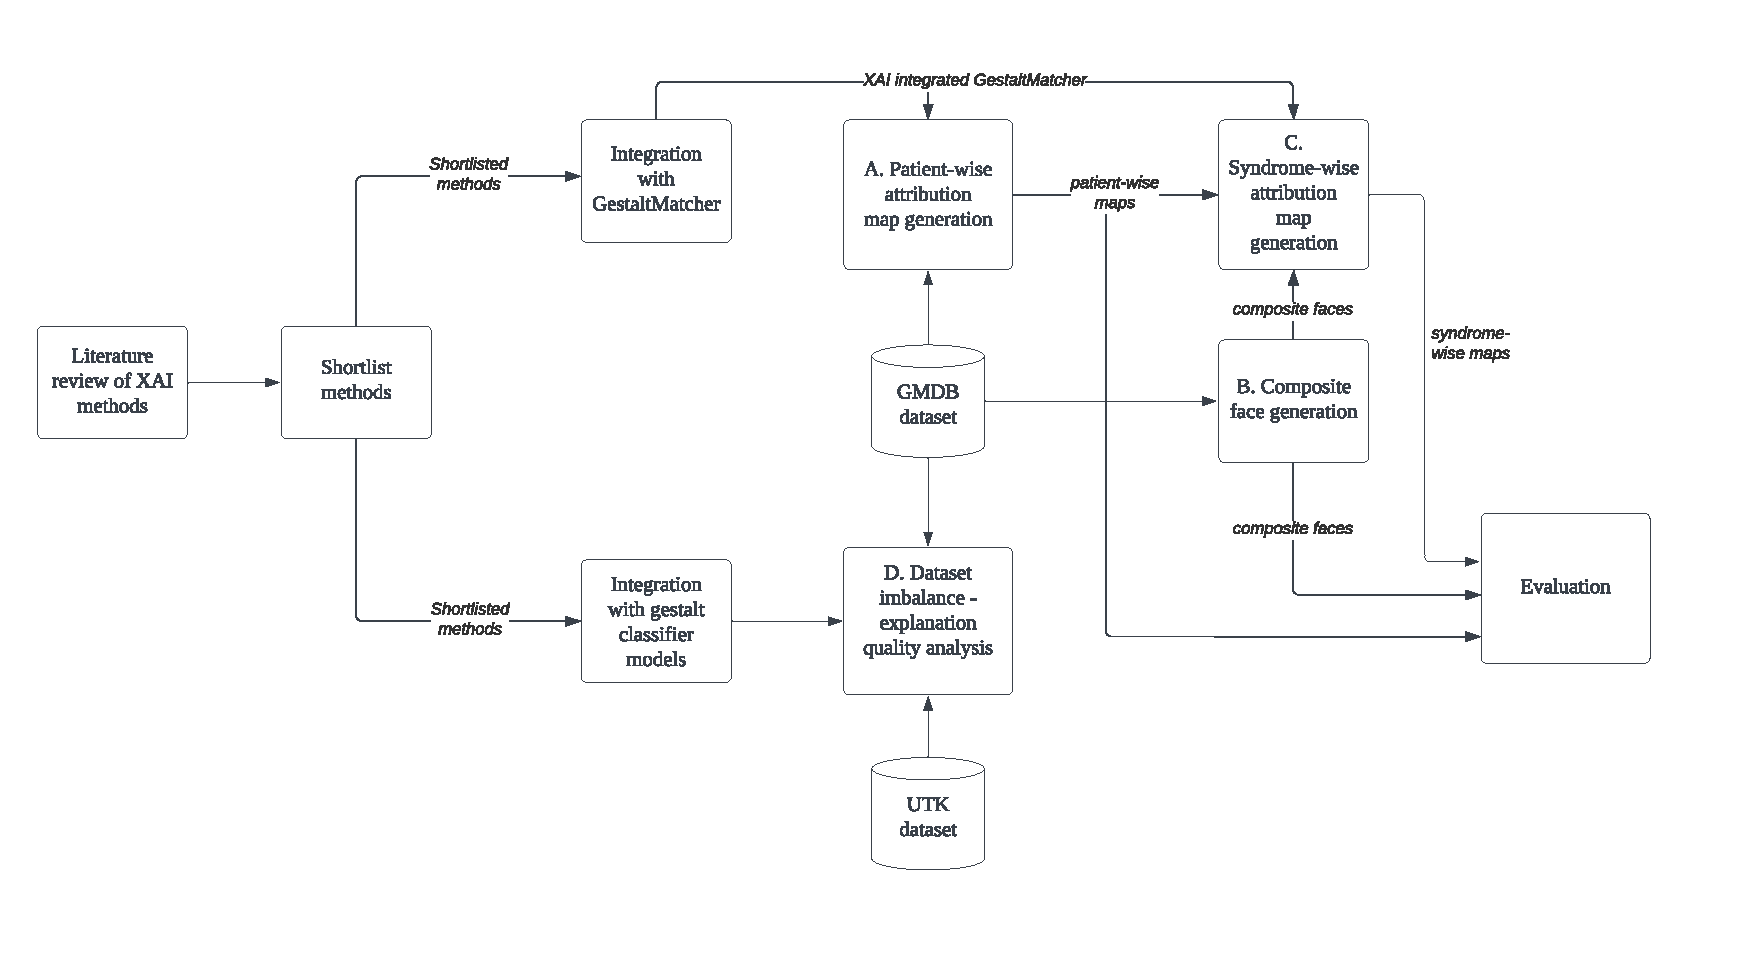
\includegraphics[scale=0.62]{chapter4/experiment_design.pdf}
        	\caption{Design of experiments}
    	    	\label{fig_exp_design}
    \end{figure}
    Figure \ref{fig_exp_design} illustrates the methodical approach taken to realize the objectives of this research work. The previous chapter and Section \ref{sec_method_selection} discussed the XAI methods considered for this work and explained the rationale to select three of them for further experimentation. The next step is to integrate the selected set of methods with the GestaltMatcher model, on which the planned experiments are conducted. 

    \subsubsection{A. Patient-wise Attribution Maps Generation}
    This experiment focuses on one of our research objectives, to use XAI methods to generate explanations for individual predictions produced by the GestaltMatcher model. 
    Patient-wise attribution maps help us in knowing GestaltMatcher's attention regions in every patient face from GMDB dataset. In turn, this helps us to study the patterns (if there is any) behind the model's varying regions of interests for different categories of inputs.
    \subsubsection{B. Composite Face Generation}
    Experiments B and C are conducted with an intent to obtain a characteristic representation of GestaltMatcher's regions of interest in a syndrome(class)-wise manner. Composite face representation of a given class is obtained by applying certain image transformations and averaging patient faces belonging to it (see \ref{} Chapter 5 for the detailed description). Thus generated composite faces are then processed by the XAI integrated GestaltMatcher model to produce its corresponding attribution maps using all three selected methods.
    \subsubsection{C. Syndrome-wise Attribution Maps Generation}
    Although, attribution maps of composite faces are generated with an intent to give a generic representation, they suffer from a couple of drawbacks. The process of applying image transformations to facial images of patients to generate composite faces, may alter the key facial abnormalities and dysmorphic features associated with corresponding genetic syndromes. Besides, there is a possibility of the GestaltMatcher model to misclassify them, raising concerns about the correctness of generated attribution maps. 
    
    In order to overcome these challenges, we propose and deploy two other techniques to produce syndrome-wise attribution maps: averaging and Singular Value Decomposition (SVD). These techniques are applied to only attribution maps associated with correctly predicted inputs. However, syndrome-wise attribution maps generated using all the three techniques are considered for evaluation, provided the composite face of a given syndrome is correctly predicted.
    \subsubsection{D. Dataset Imbalance - Explanation Quality Analysis} \label{sec_data_imb}
    As discussed in Section \ref{sec_challenges}, GMDB dataset is imbalanced. We hypothesize that the problem could affect the quality of attribution maps generated from the GestaltMatcher model. This experiment verifies the hypothesis.\\
    We train three different classifier models: two trained with balanced sets of classes, and one with an imbalanced set. We observe and analyze the changes in attribution maps produced from these models. Besides this investigation, we study the variations in GestaltMatcher's regions of attention in syndromic and healthy faces. This is realized by analyzing attribution maps produced from a binary classifier, which is trained to differentiate faces of syndromic and healthy individuals. Facial images of healthy people are obtained from the UTKFace dataset.
    \section{Evaluation}\label{sec_evaluation}
    Evaluating XAI methods based on their explanation correctness remains a challenge till date. Yeh \etal \cite{yeh2019fidelity} classifies explanation evaluation measures into two categories: objective or computational measures and subjective measures. Objective measures evaluate explanations based on whether a given XAI method satisfies certain properties or axioms, such as completeness\cite{sundararajan2017axiomatic}. On the other hand, subjective measures focus on aspects such as explanation usefulness, and the evaluation procedure involves humans. This research work uses subjective measures to evaluate the explanation artifacts produced by the chosen set of XAI methods.\\ 
    In the beginning, this section briefly explains the two predominantly used objective measures to evaluate saliency mapping methods: \enquote{infidelity and sensitivity}\cite{yeh2019fidelity}, to give the reader an idea about what computational metrics typically look for. Subsequently, the rationale behind using subjective measures over objective ones for this work is provided. Finally, the proposed evaluation procedure is described in detail.
    \subsection{Objective Measures}
    Yeh \etal \cite{yeh2019fidelity} proposed infidelity and sensitivity metrics in their work, to benchmark various saliency mapping methods. These measures are computed based on the changes observed in model explanations, when its inputs are subject to perturbations. 
    \subsubsection{Infidelity}
    \begin{equation}
    	content...
    \end{equation}
    Infidelity computes the expected mean squared difference between an explanation scaled by the magnitude of an input perturbation, and differences between the predictor function of the given model at its input and perturbed input. Intuitively, this refers to the correctness of an XAI method in generating true explanations for model predictions.
    \subsubsection{Sensitivity}
    \begin{equation}
    	content...
    \end{equation}
    Sensitivity can explained as the change in model explanation resulting from a small perturbation in the input.
    
    \subsection{Rationale to Adopt Subjective Evaluation}
    Although, computational measures such as the ones presented offer a quantitative means to benchmark XAI methods, they cannot be used for evaluating them on abstract objectives such as meaningfulness of explanations. Such an evaluation can only be performed in subjective manner, by end users of the AI system.\\
    Mohseni \etal \cite{mohseni2021multidisciplinary} list various possible goals with which XAI methods can be used, and also recommend measures to evaluate them, based on the context of their application. The goals listed in their work are as follows: algorithmic transparency, user trust and reliance, bias mitigation, privacy awareness, model visualization and inspection, model tuning and selection, model interpretability and debugging.\\ 
    The primary goals of this research work can be related to three of the above mentioned: \enquote{algorithmic transparency}, \enquote{user-trust and reliance} and \enquote{model interpretability}. For such cases, authors recommend to evaluate XAI methods by conduct human-subject studies using tools such as Likert-scale questionnaires \cite{likert_scale}. This research work follows the recommendation, and formulates a questionnaire for clinicians (end-users) to evaluate the generated explanations. 
    \subsection{Proposed Evaluation Procedure}
    The three types of artifacts (patient-wise map, composite face and syndrome-wise map) generated from the above mentioned experiments are meant to be evaluated by clinicians, who are familiar with the syndromes in our scope. This research work formulates evaluation procedures for each artifact. Clinical practitioners were consulted to develop the procedures. The proposed evaluation strategies are realized in the form of a questionnaire, which is presented in \ref{} Chapter 5. 
    \subsubsection{i. Patient-wise Attribution Maps}
    Steps to evaluate patient-wise maps are presented in Figure \ref{fig_patient_flow} as a flowchart. Besides illustrating the process flow, the chart enumerates possible responses and what can be inferred from them. Scenarios B and C are desirable, as they indicate the usefulness of attribution maps. The final step ranks attribution maps generated by the four chosen methods based on their usefulness.
    
    It is important to note that this evaluation procedure is performed on attribution maps of correctly predicted test samples from GMDB dataset. The idea to evaluate attribution maps of test instances is based on the recommendation from Molnar in his book titled \enquote{Interpretable Machine Learning}\cite{molnar2019}.
    
     \begin{figure}[H]
     	\hspace*{1cm}    
    	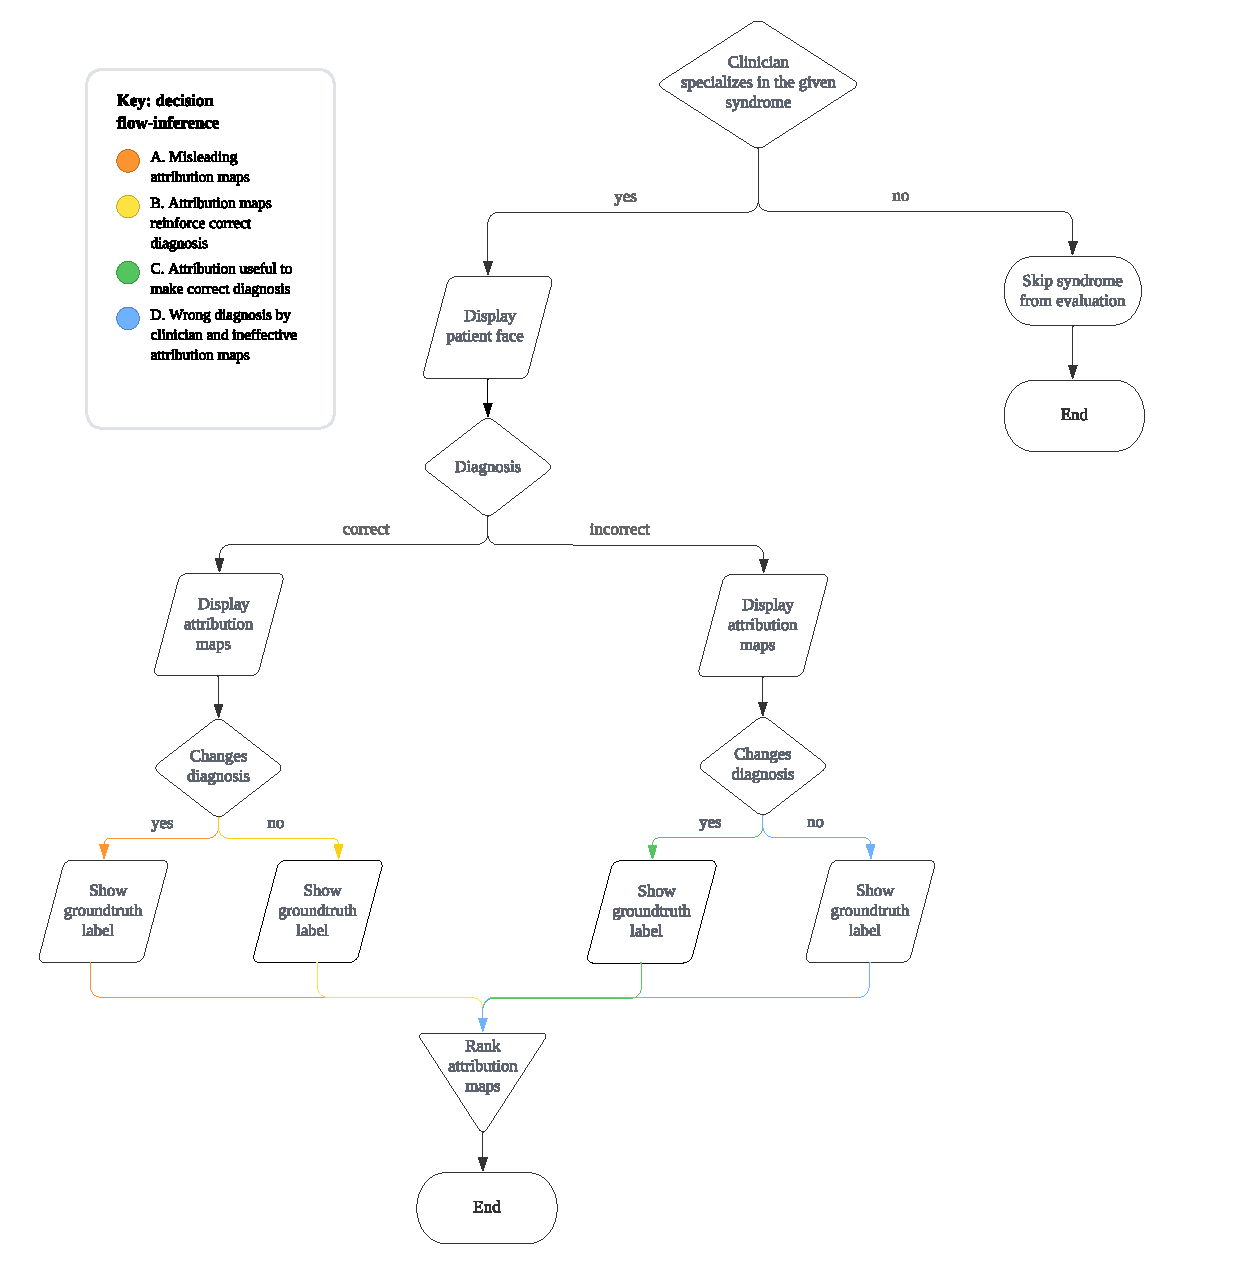
\includegraphics[scale=0.7,trim = 0cm 1cm 0cm 0cm]{chapter4/patient_wise_tree.pdf}
    	\vspace*{1cm}
   	    \caption{Proposed procedure to evaluate patient-wise attribution maps}
		\label{fig_patient_flow}
    \end{figure}

	\subsubsection{ii. Composite Faces}
	The implicit goal of evaluating composite faces is to know if they contain all or most of characteristic facial features of a genetic syndrome. Unlike the case of individual patient images, ground truth labels associated with composite faces are not known before hand, as they are synthesized using facial features from multiple images of a class. Therefore, at first it is important to know whether a given composite face atleast resembles a patient face of a particular syndrome, before looking for its prominent features. The same idea is illustrated as a flowchart in Figure \ref{fig_composite_flow}. 
	
	\begin{figure}[H]
		\hspace*{1cm}      
		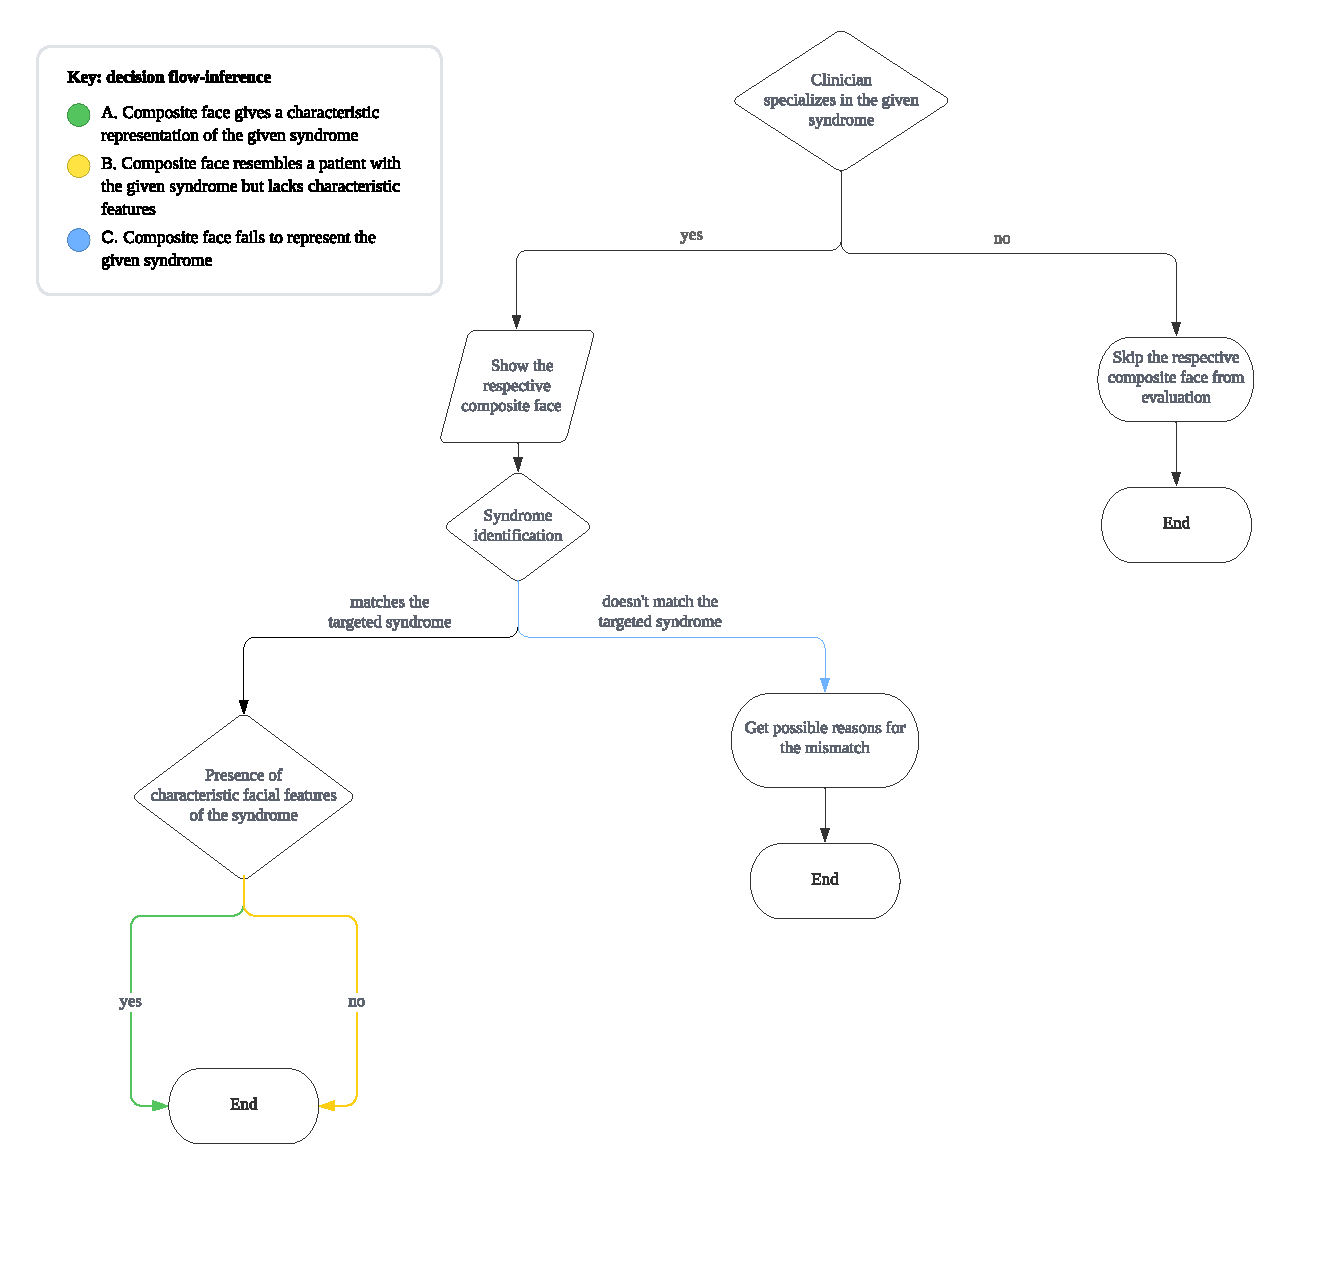
\includegraphics[scale=0.6,trim = 0cm 7cm 0cm 0cm]{chapter4/composite_face_tree.pdf}
		\vspace*{4cm}
		\caption{Proposed procedure to evaluate composite faces}
		\label{fig_composite_flow}	
	\end{figure}

	\subsubsection{iii. Syndrome-wise Attribution Maps}
	Syndrome-wise attribution maps are evaluated in a single step process. The target syndrome is revealed, and the evaluator is asked to pick top three attribution maps, based on how well they highlight the facial regions containing all or most of the disorder's features.
	
	
	\begin{figure}[H]
		\hspace*{4.5cm}      
		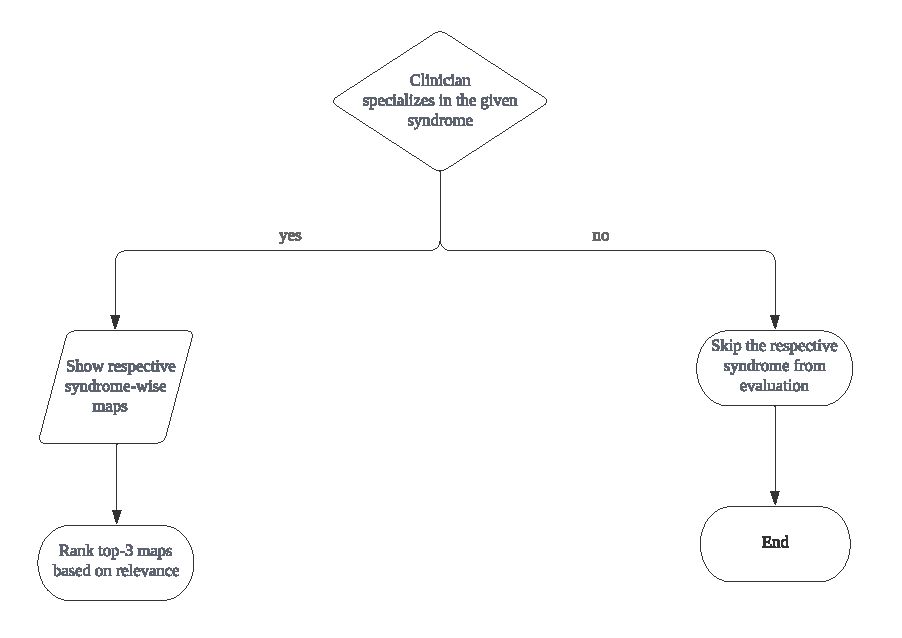
\includegraphics[scale=0.55]{chapter4/syndrome_wise_tree.pdf}
		\caption{Proposed procedure to evaluate composite faces}
		\label{fig_composite_flow}	
	\end{figure}
\end{document}
